\documentclass{article}
\usepackage{authblk}
\usepackage[T1]{fontenc}
\usepackage[utf8]{inputenc}
\usepackage{graphicx}
\usepackage{listings}
\usepackage{placeins}
\usepackage{amssymb}

\title{Recursion, Game Trees and Classes - Making an unbeatable algorithm.}

\author[]{Tushar Rakheja}
\author[]{Shibjash Dutt}
\author[]{Hanit Banga}

\affil[]{\texttt{Instructors @ Endofline Computer Club}}

\renewcommand\Authands{ and }

\date{August 2015}

\begin{document}

\maketitle

\section{Introduction}

In the last session, we talked about functions. We'll start this session by talking about recursive functions. These are functions that refer to themselves, in order to compute what they're meant to. We'll discuss the theory, some classic examples, and some interesting questions that are recursive in nature. \\

\noindent After that, we'll take a slight detour into programming and learn about lists in Python. A list is a data structure \cite{DSinPres_Slide} that stores elements sequentially.\\

\noindent Once we're done with lists, we'll come back to Tic-Tac-Toe, but this time we'll look at it with little to no code. We'll then introduce the tree data structure, and the class programming construct. Finally, we'll put all of it together, and assemble the Earth's Mightiest Zeros. 

\section{Recursive Functions}

\noindent So far, we've seen that a function is just a set of instructions in a program that can be called to perform the same set of instructions on different \textit{arguments}. Even though this seems like a simple thing, a cleverly designed function can perform awefully complex computations depending upon the argument. It's a necessary tool for a programmer. You'll see. Let's see what we mean by introducting the concept of \textit{recursive functions}. \\

\noindent Recursive functions, in many ways, are just like normal functions. They take in some arguments and perform a series of instructions. However, there's one key difference - one of these intructions in a recursive function is a call to itself. \\

\noindent "... wait, what?" Yeah, we know. A recursive function calls itself, you read it right. And when it calls itself, it again calls itself as a part of the call (since it performs the same series of instructions - it's the same function after all). Doesn't that sound like an infinite loop? It may, but it isn't of course. Each time a recursive function calls itself, something changes, which eventually stops this otherwise endless self-calls - \underline{the argument}. \\

\noindent A recursive function has something called a \underline{base case} or an \underline{end condition}, that depends upon the argument. When the argument attains a certain value, the base case is triggered, and the function doesn't call itself again. (As you may have guessed, this base case is checked using an if\{ \} block) Before saying anything else, let's look at an example - let's write a function to multiply two integers, $a$ and $b$. \\

\noindent \underline{\textit{Version 1: Non-recursive}} 
\begin{lstlisting}[language=Python]

def mult(a, b):     
    return a*b 
    
\end{lstlisting} 
\vspace{5mm}

\noindent \underline{\textit{Version 2: Recursive}} 
\begin{lstlisting}[language=Python]

def mult(a, b):
    if (b == 0):
        return 0
    else:
        return a + mult(a, b-1)
        
\end{lstlisting}
\vspace{5mm}

\noindent This example was terribly trivial (especially Version 1, to the point of being unnecessary). But, do you see how Version 2 works? On the next page there's a visualization with $a = 3$ and $b = 4$. Follow the small black arrows first, paying attention only to things in black. Once you reach the end, follow the red arrows back up along with the explanation. Each function call looks like this: 

\FloatBarrier
\begin{figure}
    \centering
    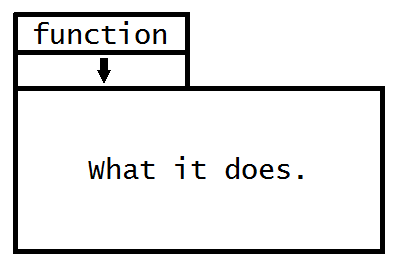
\includegraphics[scale=0.5]{SampleFunction}
    \caption{Sample Function.}
    \label{SampleFunction}
\end{figure}
\newpage 

\begin{figure}
    \centering
    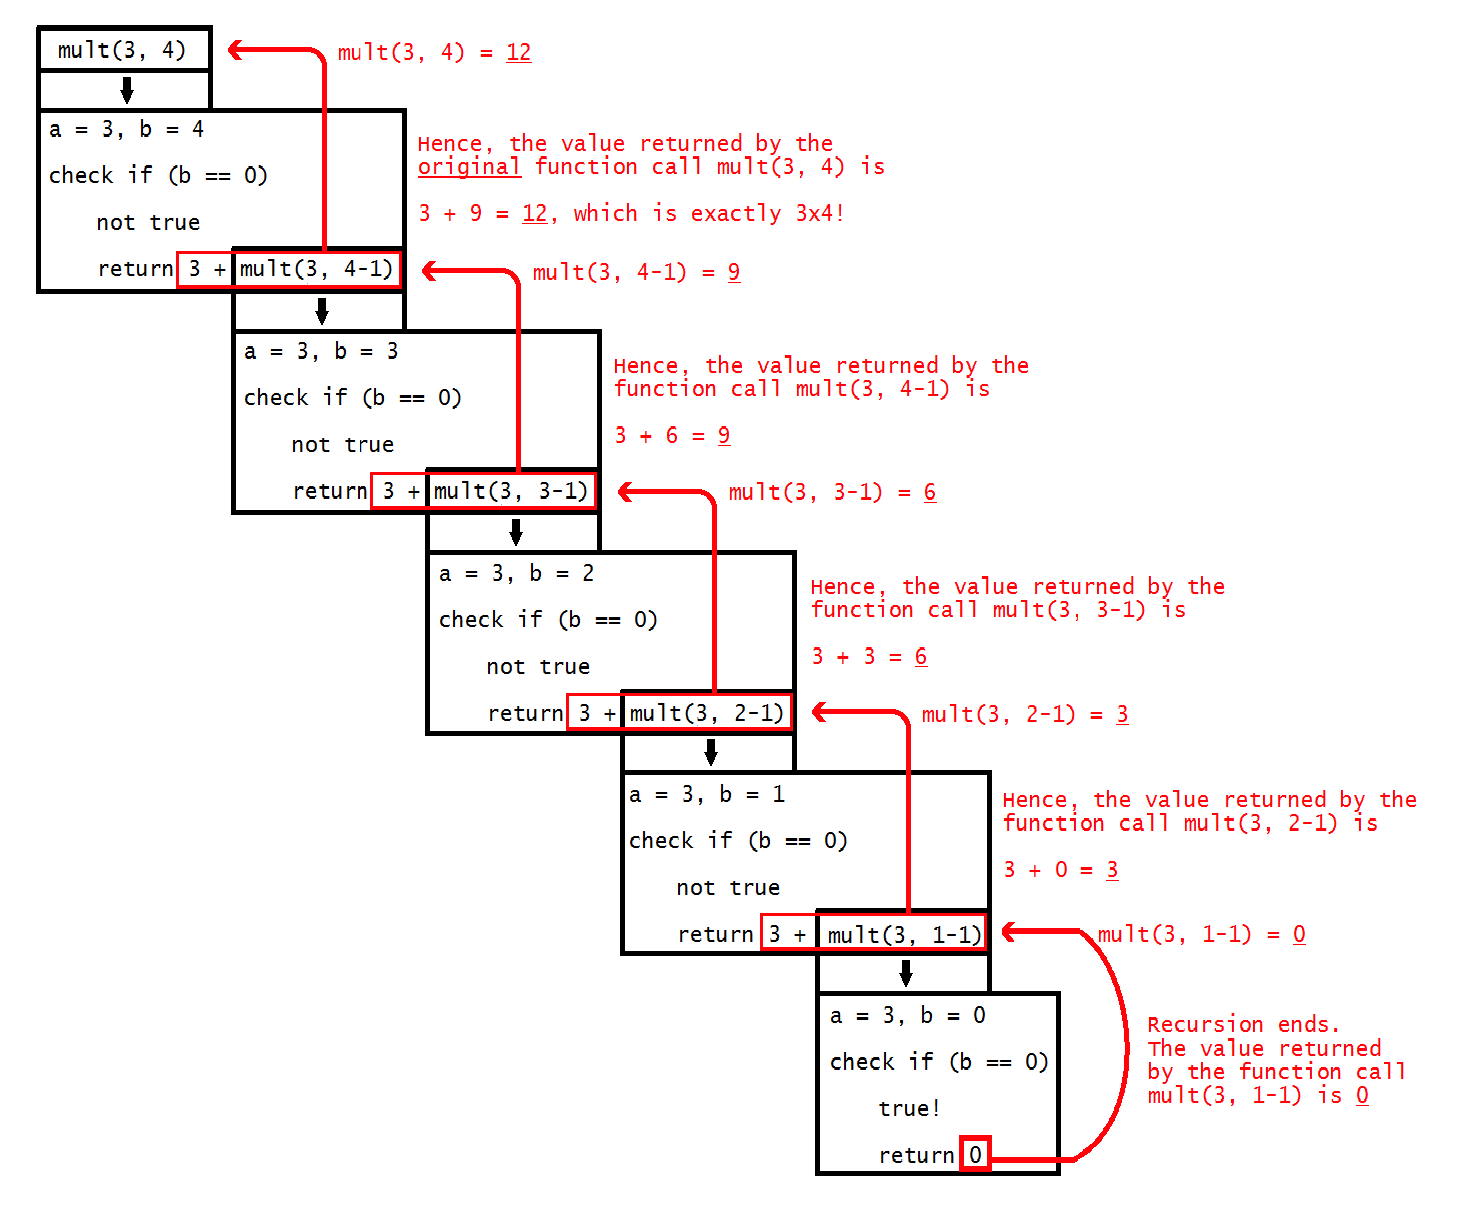
\includegraphics[scale=0.415]{Recursion}
    \caption{Visualizing mult(3, 4), Version 2.}
    \label{Recursion}
\end{figure}
\FloatBarrier

\noindent Hopefully that example made it very clear what recursion is. In a way, you could compare the example with \textit{iteration}, or, in programming, the class of constructs called \textit{loops}. It's a very valid parallel to draw.\\

\noindent However, even though there are many instances where a problem that can be solved using iteration can also be solved using recursion (and vice versa), there's a certain sense in which recursion and iteration seem, fundamentally different.

\begin{itemize}
\item The basic idea behind \underline{iteration} is to:
    \begin{enumerate}
    \item Identify that the problem involves performing a \textit{similar series of steps} on the data. 
    \item Note that the data has an inherently sequential structure, which can be exploited to solve the problem. 
    \item Perform all those steps \textit{serially} on the data, and stop when we're done (that is, a certain condition is reached). 
    \end{enumerate}
\item The basic idea behind \underline{recursion} is to:
    \begin{enumerate}
    \item Break down a problem into successively smaller and smaller problems.
    \item Compute the solution to the smallest possible problems that can be \textit{easily} solved (the \textit{base} case), and 
    \item Finally combine the solutions to the smaller problems to get solutions for successively bigger ones - and eventually, for the biggest (original) one. 
    \end{enumerate}  
\end{itemize}

\noindent There are several obvious differences. Can you think of some of them? Just off the top of your head. It's an interesting thing to think about. Here's an analogy. Say you want to calculate this product: $2\cdot 3\cdot 4\cdot 5$. 

\begin{itemize}
\item Say you decide to follow these steps.
    \begin{enumerate} 
    \item \ \ \ \ $2\cdot 3 = 6$. 
    \item \ \ \ \ $6\cdot 4 = 24$.
    \item \ \ \ \ $24\cdot 5 = 120$.
    \end {enumerate}
    And done.
\item Alternatively, you could just as well do. 
    \begin{enumerate}
    \item \ \ \ \ $2\cdot 3 = 6$.
    \item \ \ \ \ $4\cdot 5 = 20$.
    \item \ \ \ \ Combining the first two steps, $6\cdot 20 = 120$.
    \end{enumerate}
    And done too!
\end{itemize}

\noindent See? Two different approaches to solving the same problem. Here, the distinction between an iterative approach and a recursive approach is even starker. It would be more so, say, if we had $2^10$ numbers that we wanted to multiply. \\

\noindent What we gave you is a very CS-centric view of recursion. Howver, recursion is not fundamentally a programming construct. It's very well defined mathematically too, and that foundation is often useful in CS, especially in the study of algorithms that work recursively. You'll be surprised to know that some of the most efficient algorithms that we know of, are recursive in nature - they are often called \textit{divide and conquer} algorithms. \\

\noindent Here, check out these Wikipedia articles on Recursion\cite{Recursion in CS} and the Divide and Conquer paradigm\cite{Divide and Conquer}. \underline{Detour}: In fact, whenever you start learning something new - anything, a new software, a programming language, a new poem, whatever - it's always good to know a little about the story and history of the thing. Even though you may not understand everything, or even most things, it'll only add to your experience. \\

\noindent Just for closure, let's talk a bit about a mathematical function that is often defined recursively. 

\subsection{Factorial} 

\noindent This is quite the archetype of a recursively defined mathematical function. It takes in a single argument, $n$, and returns the product of all the natural numbers from $1$ to $n$ (both inclusive). By convention, we denote the factorial of $n$ by $n!$, and $0! = 1$. Here's the formal definition. 

\begin{displaymath}
    n! = \left\{
    \begin{array}{lr}
        1 & \ \ n = 0\\
        n\cdot (n-1)! & \ \ n \neq 0\\
    \end{array}
    \right.
\end{displaymath} 

\noindent \underline{Exercise}: Try to make a recursion graphic, similar to the one shown earlier in the document, for $n!$ ($n \in \mathbb{N}$). You can find a lot more on the internet about the factorial than what can be presented here. Be sure to check it out. \\

\noindent This ends our discussion about recursive functions, for now. If you wish to delve deeper into the details, please do so! Let's now continue to build our toolkit. Let's talk about lists. 

\section{Lists}

Lists in Python are pretty much what you'd expect them to be. Lists. They can contain anything, with some sense of order. 

A list is a simple \textit{data structure}, and like every data structure, it has an API, or a set of things it can do for you. Here's the only part of its API we'll need. 

\begin{itemize}
    \item Initialize: You can initialize an empty list this way: 
        \begin{lstlisting}[language=Python]
        >>> example = [] # 'example' is the name of the list.
        \end{lstlisting}
    Of course, the list list doesn't have to be empty:
        \begin{lstlisting}[language=Python]
        >>> example = ['TRex', 1]
        \end{lstlisting}
    \item Append: You can append (insert at the end of the list) a certain element. Consider the nonempty initialized list in the previous point: 
        \begin{lstlisting}[language=Python]
        >>> example.append(2)
        >>> example 
        ['TRex', 1, 2]
        \end{lstlisting}
    \item Remove: Actually, we may not even need remove, but one should know how to undo what they've done.
        \begin{lstlisting}[language=Python]
        >>> example.remove(1)
        ['TRex', 2]
        \end{lstlisting}
    \item Length
    \item Contains
\end{itemize}


\section{Trees}

\section{Game states} 

So far, we've looked at various tools, like functions, recursion and lists,
which will help us in our analysis of the game. Let us now start working with
a more concrete idea, that of \textit{game states}. \\

\noindent Imagine a game of Tic-Tac-Toe played between Alice and Bob. Alice is playing crosses (X) and Bob is playing zeros (O). \\

\noindent Here is an example of how such a game might proceed, if Alice plays first:

\begin{center}
    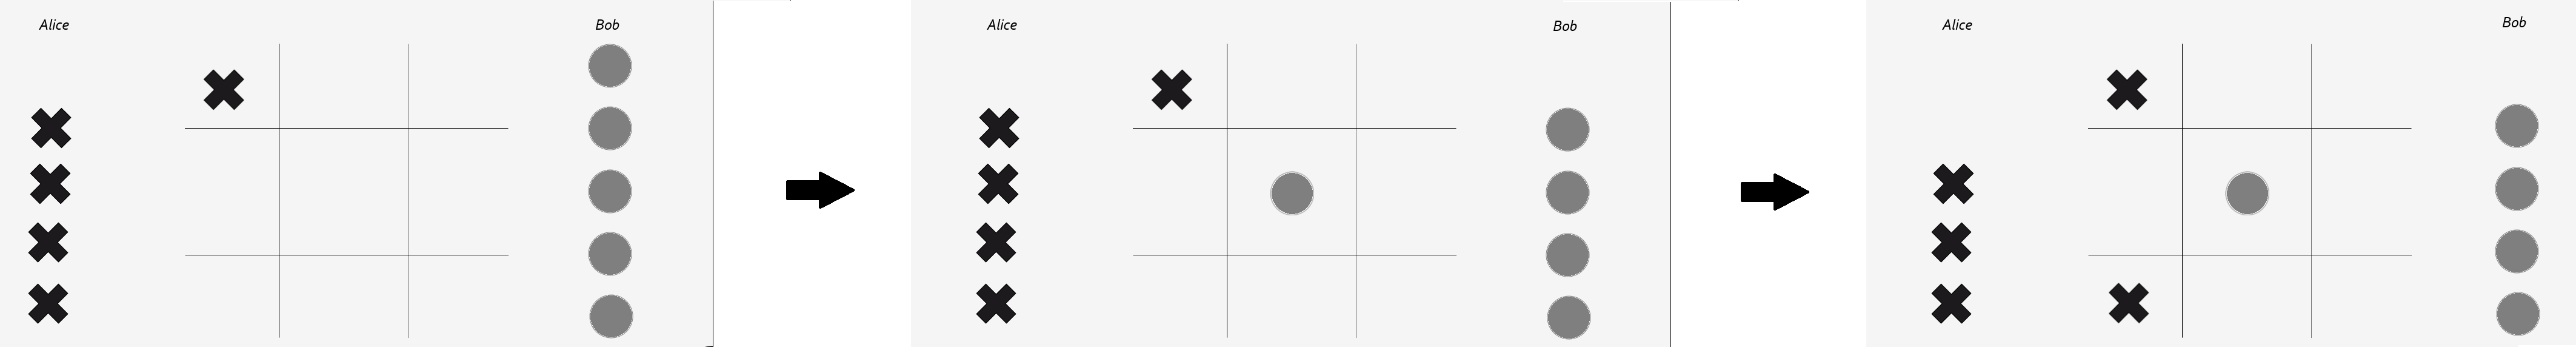
\includegraphics[scale=0.11]{AliceVBob}
\end{center}

\noindent And so on. \\

\noindent A \textit{game state} is, predictably, the \textit{state} or the configuration of the game, at some particular time. As far as Tic-Tac-Toe is concerned, we could define the game state to be the "contents" of the board and their respective locations at some time \textit{t}. \\

\noindent Informally, the game state is a "snapshot" or a "photograph" of the board at some time. A simple concept, but why's it useful? Let's see. 

\section{Classes}

\section{Putting it all together}

\subsection{Game Trees}

\subsection{Relating game states to game trees}

\begin{thebibliography}{9}
\bibitem{DSinPres_Slide} {
Tushar Rakheja and Shibjash Dutt.
\textit{"CS. What it is, what it isn't, and why you should care."}
\texttt{https://github.com/EndoflineComputerClub/TicTacTongue.}
\\PresentationCS.pptx, slide 11. }

\bibitem{Recursion in CS} 
Wikipedia.
\textit{Recursion (computer science) - Wikipedia, the free encyclopedia}
\texttt{https://en.wikipedia.org/wiki/Recursion\_(computer\_science)}

\bibitem{Divide and Conquer} 
Wikipedia.
\textit{Divide and conquer algorithms - Wikipedia, the free encyclopedia}
\texttt{https://en.wikipedia.org/wiki/Divide\_and\_conquer\_algorithms}
\end{thebibliography}

\end{document}